\label{ch:multigrid}

\begin{quote}
\noindent {\em These summarize multigrid on cell-centered grids.  The
  text ``A Multigrid Tutorial''~\cite{multigridtutorial} is an incredible
  reference.  These notes discuss the basics and point out some specific
  details for cell-centered grids.}
\end{quote}

\section{Elliptic equations}

The simplest elliptic PDE is {\em Laplace's equation}:
\begin{equation}
\nabla^2 \phi = 0
\end{equation}
Only slightly more complex is {\em Poisson's equation} (Laplace + a source term):
\begin{equation}
\nabla^2 \phi = f
\end{equation}
These equations can arise in electrostatics (for the electric potential),
solving for the gravitational potential from a mass distribution, or
enforcing a divergence constraint on a vector field (we'll see this
when we consider incompressible flow).

Another common elliptic equation is the {\em Helmholtz equation}:
\begin{equation}
(\alpha - \nabla \cdot \beta \nabla) \phi = f
\end{equation}
A Helmholtz equation can arise, for example, from a time-dependent
equation (like diffusion) by discretizing in time.

Notice that there is no time-dependence in any of these equations.
The quantity $\phi$ is specified instantaneously in the domain subject to
boundary conditions.

\section{FFTs}

A direct way of solving a constant-coefficient elliptic equation
is using Fourier transforms.  Using a general Fourier transform
(which we consider here) works only for periodic boundary conditions,
but other basis functions can be used for other boundary conditions.

Consider the Poisson equation:
\begin{equation}
\nabla^2 \phi = f
\end{equation}
We will difference this in a second-order accurate fashion.  Thinking
of the Laplacian as $\nabla^2 \phi$ = $\nabla \cdot \nabla \phi$, we
first compute the gradient of $\phi$ on edges:
\begin{equation}
[\nabla \phi \cdot \hat{x}]_{i+1/2,j} = \frac{\phi_{i+1,j} - \phi_{i,j}}{\Delta x}
\end{equation}
Since this is defined on edges, this represents a centered difference, and is
therefore second-order accurate.  We then difference the edge-centered
gradients to the center to get the Laplacian at cell-centers:
\begin{align}
[\nabla^2 \phi]_{i,j} &=
   \frac{[\nabla \phi \cdot \hat{x}]_{i+1/2,j} -
         [\nabla \phi \cdot \hat{x}]_{i-1/2,j}}{\Delta x} +
   \frac{[\nabla \phi \cdot \hat{y}]_{i,j+1/2} -
         [\nabla \phi \cdot \hat{y}]_{i,j-1/2}}{\Delta y} \nonumber\\
%
  &= \frac{\phi_{i+1,j} - 2\phi_{i,j} + \phi_{i-1,j}}{\Delta x^2} +
     \frac{\phi_{i,j+1} - 2\phi_{i,j} + \phi_{i,j-1}}{\Delta y^2} = f_{i,j}
\end{align}        
Again, since we used a centered-difference of the edge values, this
expression is second-order accurate.  This is the standard
{\em 5-point stencil} for the 2-d Laplacian.

We now assume that we have an FFT subroutine that can take our
discrete real-space data, $\phi_{i,j}$ and return the discrete
Fourier coefficients, $\phi_{k_x,k_y}$.

We now express $\phi_{i,j}$ and $f_{i,j}$ as sums over their Fourier
components.  Note, because we are using $i$ as the grid index, we will
use $\imag$ as the imaginary unit:
\begin{align}
\phi_{i,j} &= \frac{1}{MN} \sum_{k_x = 0}^{M-1} \sum_{k_y = 0}^{N-1}
  \Phi_{k_x,k_y} e^{2\pi\imag i k_x/M} e^{2\pi\imag j k_y/N} \\
f_{i,j} &= \frac{1}{MN} \sum_{k_x = 0}^{M-1} \sum_{k_y = 0}^{N-1}
  F_{k_x,k_y} e^{2\pi\imag i k_x/M} e^{2\pi\imag j k_y/N} 
\end{align}

Inserting these into the differenced equation (and dropping the sums
and normalization, to focus on a single mode), we have:
\begin{align}
\frac{1}{MN}\sum_{k_x=0}^{M-1}\sum_{k_y=0}^{N-1}
\biggl \{
&\frac{\Phi_{k_x,k_y}}{\Delta x^2} e^{2\pi\imag j k_y/N}
  \left [ e^{2\pi\imag (i+1) k_x/M} -2 e^{2\pi\imag i k_x/M} +
         e^{2\pi\imag (i-1) k_x/M} \right ] + \nonumber \\
&\frac{\Phi_{k_x,k_y}}{\Delta y^2} e^{2\pi\imag i k_x/M}
  \left [ e^{2\pi\imag (j+1) k_y/N} -2 e^{2\pi\imag j k_y/N} +
         e^{2\pi\imag (j-1) k_y/N} \right ] \biggr \} = \nonumber \\
\frac{1}{MN}\sum_{k_x=0}^{M-1}\sum_{k_y=0}^{N-1}
 & F_{k_x,k_y} e^{2\pi\imag i k_x/M} e^{2\pi\imag j k_y/N}
\end{align}

We can bring the righthand side into the sums on the left, and we can
then look at just a single term:
\begin{align}
  e^{2\pi\imag i k_x/M} e^{2\pi\imag j k_y/N}
  \biggl \{
  &\frac{\Phi_{k_x,k_x}}{\Delta x^2}
  \left [e^{2\pi\imag k_x/M} + e^{-2\pi\imag k_x/M} - 2 \right ] + \nonumber \\
  &\frac{\Phi_{k_x,k_x}}{\Delta y^2}
  \left [e^{2\pi\imag k_y/N} + e^{-2\pi\imag k_y/N} - 2 \right ] 
  - F_{k_x,k_y}
  \biggr \} = 0
\end{align}
Simplifying, we have:
\begin{equation}
  \Phi_{k_x,k_y} = \frac{1}{2}\frac{F_{k_x,k_y}}
      {\left [\cos(2\pi k_x/M) - 1 \right ] \Delta x^{-2} +
        \left [\cos(2\pi k_y/N) - 1 \right ] \Delta y^{-2}}
      \label{eq:FFTsol}
\end{equation}
This is the algebraic solution to the Poisson equation in Fourier (frequency)
space.  Once we evaluate this, we can get the real-space solution
by doing the inverse transform.

The main downside of this approach is that, because we solve for a
single component independently (Eq.~\ref{eq:FFTsol}), this only
works for linear problems with constant coefficients.  For a problem
like:
\begin{equation}
  \nabla \cdot (\beta \nabla \phi) = f
\end{equation}
There would be ``cross-talk'' between the Fourier modes of $\beta$
and $\phi$, and we would not be able to solve for a single mode
of $\Phi_{k_x,k_y}$ independently.  We discuss methods for these
forms next.

\section{Relaxation}

Relaxation is an iterative technique, and as we will see shortly, it
provides the basis for the multigrid technique.  

Consider Poisson's equation differenced as:
\begin{equation}
\frac{\phi_{i+1,j} - 2 \phi_{i,j} + \phi_{i-1,j}}{\Delta x^2} +
\frac{\phi_{i,j+1} - 2 \phi_{i,j} + \phi_{i,j-1}}{\Delta y^2} = f_{i,j}
\end{equation}
This is a 5-point stencil: for each zone $(i,j)$, we couple in the
zones $\pm 1$ in $x$ and $\pm 1$ in $y$.  This discretization uses
the standard form for the second derivative, and is second-order
accurate in space.  

For the moment, consider the case where $\Delta x = \Delta y$.  If we
solve this discretized equation for $\phi_{i,j}$, then we have:
\begin{equation}
\phi_{i,j} = \frac{1}{4} (\phi_{i+1,j} + \phi_{i-1,j} + 
                          \phi_{i,j+1} + \phi_{i,j-1} - \Delta x^2 f_{i,j} )
\end{equation}
A similar expression exists for every zone in our domain, coupling all
the zones together.  We can't separate the solution of $\phi_{i,j}$
for the neighboring zones, but instead can apply an iterative
technique called {\em relaxation} (also sometimes called {\em
  smoothing} because generally speaking the solution to elliptic
equations is a smooth function) to find the solution for $\phi$
everywhere.  Imagine an initial guess to $\phi$: $\phi_{i,j}^{(0)}$.
We can improve that guess by using our difference equation to define a
new value of $\phi$, $\phi_{i,j}^{(1)}$:
\begin{equation}
\phi_{i,j}^{(1)} = \frac{1}{4} (\phi_{i+1,j}^{(0)} + \phi_{i-1,j}^{(0)} + 
                                \phi_{i,j+1}^{(0)} + \phi_{i,j-1}^{(0)} - 
                                 \Delta x^2 f_{i,j} )
\end{equation}
or generally, the $k+1$ iteration will see:
\begin{equation}
\phi_{i,j}^{(k+1)} = \frac{1}{4} (\phi_{i+1,j}^{(k)} + \phi_{i-1,j}^{(k)} + 
                                  \phi_{i,j+1}^{(k)} + \phi_{i,j-1}^{(k)} - 
                                   \Delta x^2 f_{i,j} )
\end{equation}
This will (slowly) converge to the true solution, since each zone is
coupled to each other zone (and to the boundary values that we need to
specify---more on that in a moment).  This form of relaxation is
called {\em Jacobi iteration}.  To implement this, you need two copies
of $\phi$---the old iteration value and the new iteration value.

An alternate way to do the relaxation is to update $\phi_{i,j}$ in
place, as soon as the new value is known.  Thus the neighboring cells
will see a mix of the old and new solutions.  We can express this in-place
updating as:
\begin{equation}
\phi_{i,j} \leftarrow \frac{1}{4} (\phi_{i+1,j} + \phi_{i-1,j} + 
                                   \phi_{i,j+1} + \phi_{i,j-1} - 
                                   \Delta x^2 f_{i,j} )
\end{equation}
This only requires a single copy of $\phi$ to be stored.  This
technique is called {\em Gauss-Seidel iteration}.  A host of other
relaxation methods exist, including linear combinations of these two.
The text by Briggs is an excellent reference for this, and discusses
the strengths of these different approaches.


Next consider the Helmholz equation with constant coefficients:
\begin{equation}
(\alpha - \beta \nabla^2) \phi = f
\end{equation}
We can discretize this as:
\begin{equation}
\alpha \phi_{i,j} - \beta \left ( 
    \frac{\phi_{i+1,j} - 2 \phi_{i,j} + \phi_{i-1,j}}{\Delta x^2} +
    \frac{\phi_{i,j+1} - 2 \phi_{i,j} + \phi_{i,j-1}}{\Delta y^2} \right )
= f_{i,j}
\end{equation}
and the update of $\phi_{i,j}$ through relaxation is:
\begin{equation}
\phi_{i,j} \leftarrow
     \left . \left ( f_{i,j} + \frac{\beta}{\Delta x^2} \phi_{i+1,j}
                             + \frac{\beta}{\Delta x^2} \phi_{i-1,j}
                             + \frac{\beta}{\Delta y^2} \phi_{i,j+1}
                             + \frac{\beta}{\Delta y^2} \phi_{i,j-1} \right ) 
\middle / \left ( \alpha + \frac{2 \beta}{\Delta x^2} + \frac{2 \beta}{\Delta y^2} \right ) \right .
\end{equation}
Notice that if $\alpha = 0$, $\beta = -1$, and $\Delta x = \Delta y$, we 
recover the relaxation expression for Poisson's equation from above.


\subsection{Boundary conditions}

When using a cell-centered grid, no points fall exactly on the
boundary, so we need to use ghost cells to specify boundary conditions.
A single ghost cell is sufficient.  The common types of boundary
conditions are {\em Dirichlet} (specified value on the boundary), {\em
  Neumann} (specified first derivative on the boundary), and periodic.
Some restrictions apply.  For example, consider $\phi_{xx} = 0$.  The
solution to this is a line, $\phi = ax + b$.  We can specify different
Neumann boundary conditions on each end, $\phi_x |_{x=x_l} = p$,
$\phi_x |_{x = x_r} = q$, because this specifies two incompatible
slopes for our line.

% created by figures/multigrid/bcs.py
\begin{figure}[h]
\centering
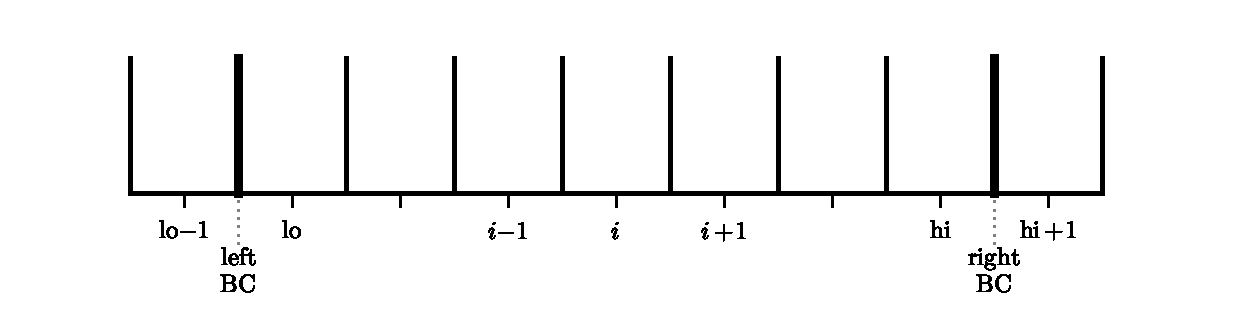
\includegraphics[width=\linewidth]{mg-bcs}
\caption[The cell-centered grid showing the difference between ghost
  cells and the physical boundary.]{\label{fig:bcs} The cell-centered
  grid showing the cells (and ghost cells) surrounding the boundaries
  and indicating that the boundary conditions are actually specified
  right at the boundary itself.}
\end{figure}

Consider Dirichlet boundary conditions, specifying values $\phi_l$ on
the left and $\phi_r$ on the right boundaries.\footnote{If the value, $\phi_l$
  or $\phi_r$ is zero, we call this a {\em homogeneous boundary condition}.  Otherwise
  we call it an {\em inhomogeneous boundary condition}}  To second order, we can
define these via:
\begin{eqnarray}
\phi_l &=& \frac{1}{2} ( \phi_\mathrm{lo} + \phi_\mathrm{lo-1} ) \\
\phi_r &=& \frac{1}{2} ( \phi_\mathrm{hi} + \phi_\mathrm{hi+1} )
\end{eqnarray}
This then tells us that the values we need to assign to the ghost cells are:
\begin{eqnarray}
\label{eq:bc_inhomo_dir}
\phi_\mathrm{lo-1} &=& 2 \phi_l - \phi_\mathrm{lo} \\
\phi_\mathrm{hi+1} &=& 2 \phi_r - \phi_\mathrm{hi}
\end{eqnarray}

If we instead consider Neumann boundary conditions, we specify values
of the derivative on the boundaries: $\phi_x |_l$ on the left and
$\phi_x |_r$ on the right.  We note that a single difference across
the boundary is second-order accurate on the boundary (it is a
centered-difference there), so to second-order:
\begin{eqnarray}
\phi_x |_l &=& \frac{\phi_\mathrm{lo} - \phi_\mathrm{lo-1}}{\Delta x} \\
\phi_x |_r &=& \frac{\phi_\mathrm{hi+1} - \phi_\mathrm{hi}}{\Delta x}
\end{eqnarray}
This then tells us that the ghost cells are filled as:
\begin{eqnarray}
\label{eq:bc_inhomo_neum}
\phi_\mathrm{lo-1} &=& \phi_\mathrm{lo} - \Delta x \, \phi_x |_l \\
\phi_\mathrm{hi+1} &=& \phi_\mathrm{hi} + \Delta x \, \phi_x |_r
\end{eqnarray}


\subsection{Residual and true error}

The {\em residual error} is a measure of how well our discrete solution
satisfies the discretized equation.  For the Poisson equation, we
can the residual as:
\begin{equation}
r_{i,j} = f_{i,j} - (L \phi)_{i,j} 
\end{equation}
and the residual error as:
\begin{equation}
\epsilon^{(r)} = \| r \|
\end{equation}
where $L$ represents our discretized Laplacian.  Note that $r$ is the
error with respect to the discrete form of the equation.  The true
error is the measure of how well our discrete solution approximates
the true solution.  If $\phi^\mathrm{true}$ satisfies $\nabla^2
\phi^\mathrm{true} = f$, then the true error in each zone is
\begin{equation}
e_{i,j} = \phi^\mathrm{true}(x_i,y_j) - \phi_{i,j} 
\end{equation}
and
\begin{equation}
\epsilon^\mathrm{true} = \| e_{i,j} \|
\end{equation}

We can make $\epsilon^{(r)}$ approach machine precision by performing
more and more relaxation iterations, but after some point, this will
no longer improve $\epsilon$.  The only way to improve
$\epsilon^\mathrm{true}$ is to make $\Delta x$ and $\Delta y$ smaller.
In practice we do not know the true solution so we cannot compute
$\epsilon^\mathrm{true}$ and will instead have to rely on
$\epsilon^{(r)}$ to monitor our error.

Note that since our operator is linear,
\begin{equation}
L e = L\phi^\mathrm{true} - L\phi = f - L\phi = r
\end{equation}
so the error in our solution obeys a Poisson equation with the residual
as the source.

\subsection{Performance}


% this figure can be created with figures/multigrid/smooth-separate.py
\begin{figure}
\centering
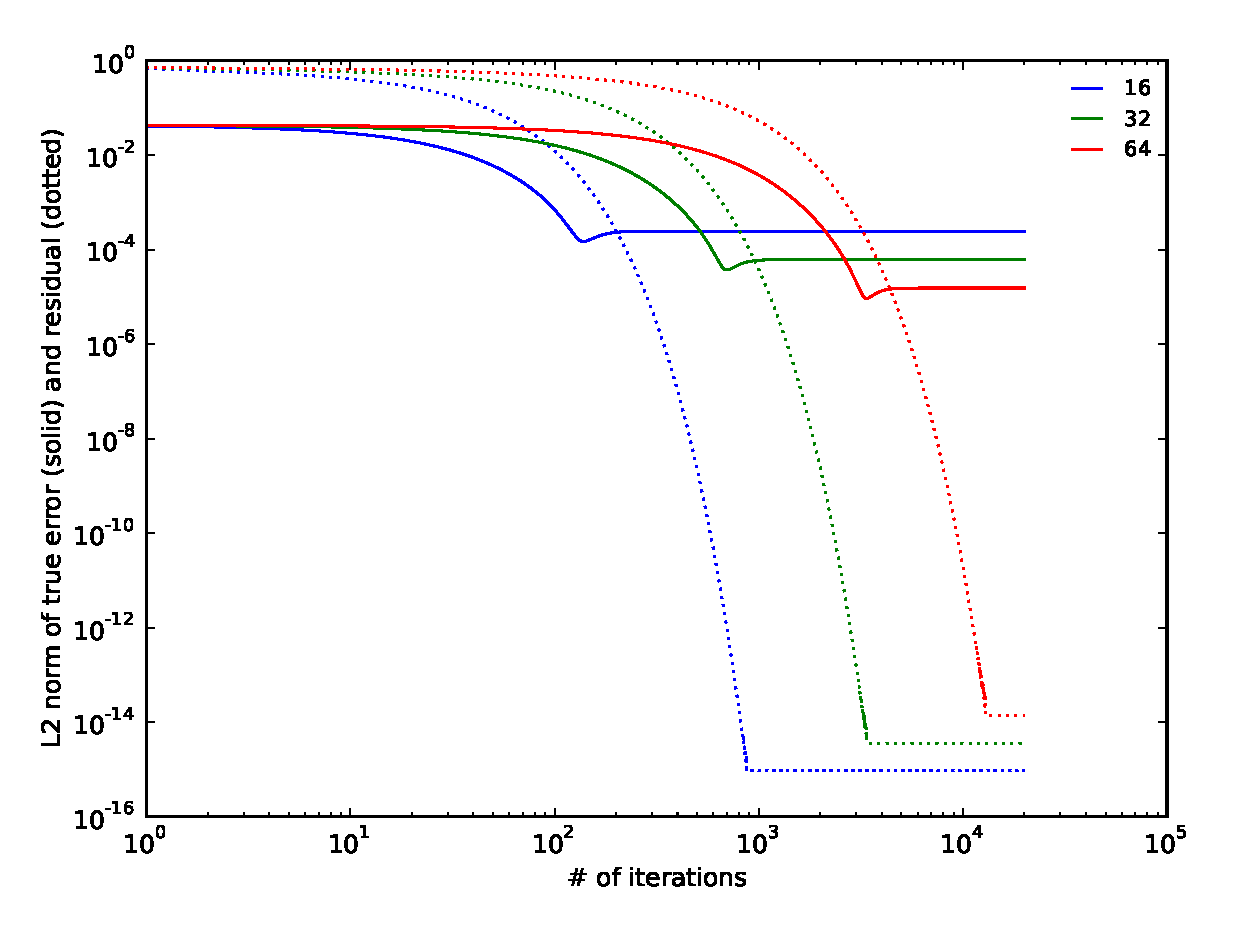
\includegraphics[width=\linewidth]{smooth-error.eps}
\caption[Convergence as a function of number of iterations using Gauss-Seidel relaxation.]{\label{fig:smootherror} Gauss-Seidel relaxation applied to
  $\phi_{xx} = \sin(x)$ with $\phi(0) = \phi(1) = 0$.  Shown are the
  L2 norm of the error compared with the true solution (solid lines)
  and the L2 norm of the residual (dotted lines) for 3 different
  resolutions (16, 32, and 64 zones).}
\end{figure}

Conside the simple Poisson problem on $x \in [0,1]$:
\begin{equation}
\phi_{xx} = \sin(x), \qquad \phi(0) = \phi(1) = 0
\end{equation}
The analytic solution to this is simply 
\begin{equation}
\phi^a(x) = -\sin(x) + x \sin(1)
\end{equation}
We can perform smoothing and compute both the error against the
analytic solution (the `true' error), $e \equiv \| \phi^a(x_i) - \phi_i \|_2$ and the
residual error, $\| r_i \|_2$.  Figure~\ref{fig:smootherror} shows these
errors as a function of the number of smoothing iterations for 3
different resolutions.

Notice that the true error stalls at a relatively high value---this is
the truncation error of the method.  From one resolution to the next,
the true error changes as $\Delta x^2$, indicating that we are
converging as our method should.  No additional amount of smoothing
will change this---we are getting the best answer to the problem we
can with our choice of discretization.

In contrast, the residual error decreases to machine precision
levels---this is indicating that our solution is an exact solution to
the discrete equation (to roundoff-error).
In practice, we can only monitor the residual error, not the true
error, and we hope that small residual error implies a small true
error.

% this figure was created with figures/multigrid/smooth_test/
\begin{figure}[t]
\centering
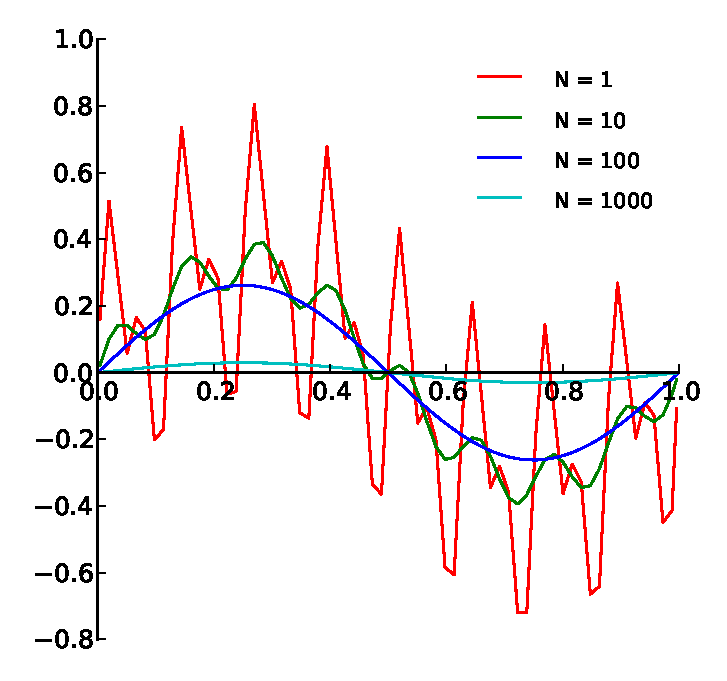
\includegraphics[width=0.8\linewidth]{smooth_error}
\caption[Smoothing of different wavenumbers.]{\label{fig:smooth} Error
  in the solution to $\phi'' = 0$ given an initial guess with 3
  different wavenumbers of noise.  The different curves are different
  numbers of smoothing iterations.}
\end{figure}

We can think of the error in the solution as a superposition of high
(short) and low (long) frequency (wavelength) modes.  Smoothing works
really well to eliminate the short wavelength noise quickly (as the
exercise shows), but many iterations are needed to remove the long
wavelength noise (see Figure~\ref{fig:smooth}).  Here the wavelength
is in terms of the number of zones across the feature, and not a
physical measure.  

\begin{exercise}[Smoothing the 1-d Laplace equation]
{Implement 1-d smoothing for the Laplace equation on
  cc-grid.  Use an initial guess for the solution:
  \begin{equation}
  \phi_0(x) = \frac{1}{3} ( \sin(2\pi x) + \sin(2\pi \, 8 x) + \sin(2\pi \, 16 x) )
  \end{equation}
  on a 128 zone grid with Dirichlet boundary conditions.  This initial
  guess has both high-frequency and low-frequency noise.  Observe that
  the high-frequency stuff goes after only a few smoothing iterations,
  but many iterations are needed to remove the low-frequency noise.
  You should see something like Figure~\ref{fig:smooth}.
}
\end{exercise}

This behavior suggests that if we could represent our
problem on a coarser grid, the error will now be of shorter
wavelength, and smoothing will be more efficient.  This is the core
idea behind multigrid.



\section{Multigrid}

The text {\em A Multigrid Tutorial}~\cite{multigridtutorial} provides
an excellent introduction to the mechanics of multigrid.  The basic
idea is to smooth a little on the current grid solving $L\phi = f$,
compute the residual, $r$, then {\em restrict} $r$ to a coarser grid and
smooth on that grid solving $Le = r$, restrict again, $\ldots$.  Once
you reach a sufficiently coarse grid, the problem solved exactly.
Then the data is moved up to the finer grids, a process called {\em
  prolongation}.  The error on the coarse grid, $e$, is prolonged to
the finer grid.  This error is then used to correct the solution on
the finer grid, some smoothing is done, and then the data is prolonged
up again.

Note: on the coarse grids, you are not solving the original system,
but rather an error equation.  If the boundary conditions in the
original system are inhomogeneous, the boundary conditions for the
error equations are now homogeneous.  This must be understood by
any ghost cell filling routines.

There are many different forms of the multigrid process.  The simplest 
is called the {\em V-cycle}.  Here you start of the fine grid, restrict
down to the coarsest, solve, and then prolong back up to the finest. 
The flow looks like a `V'.  You continue with additional V-cycles
until the residual error is smaller than your tolerance.

\subsection{Prolongation and restriction on cell-centered grids}

Multigrid relies on transferring the problem up and down a hierarchy of
grids.  Consider the following grid.  The finer grid is superposed over
the center coarse cell, and the fine grid cells are marked in red.

% this figure can be created by figures/multigrid/2dgrid-mg.py
\begin{figure}[h]
\centering
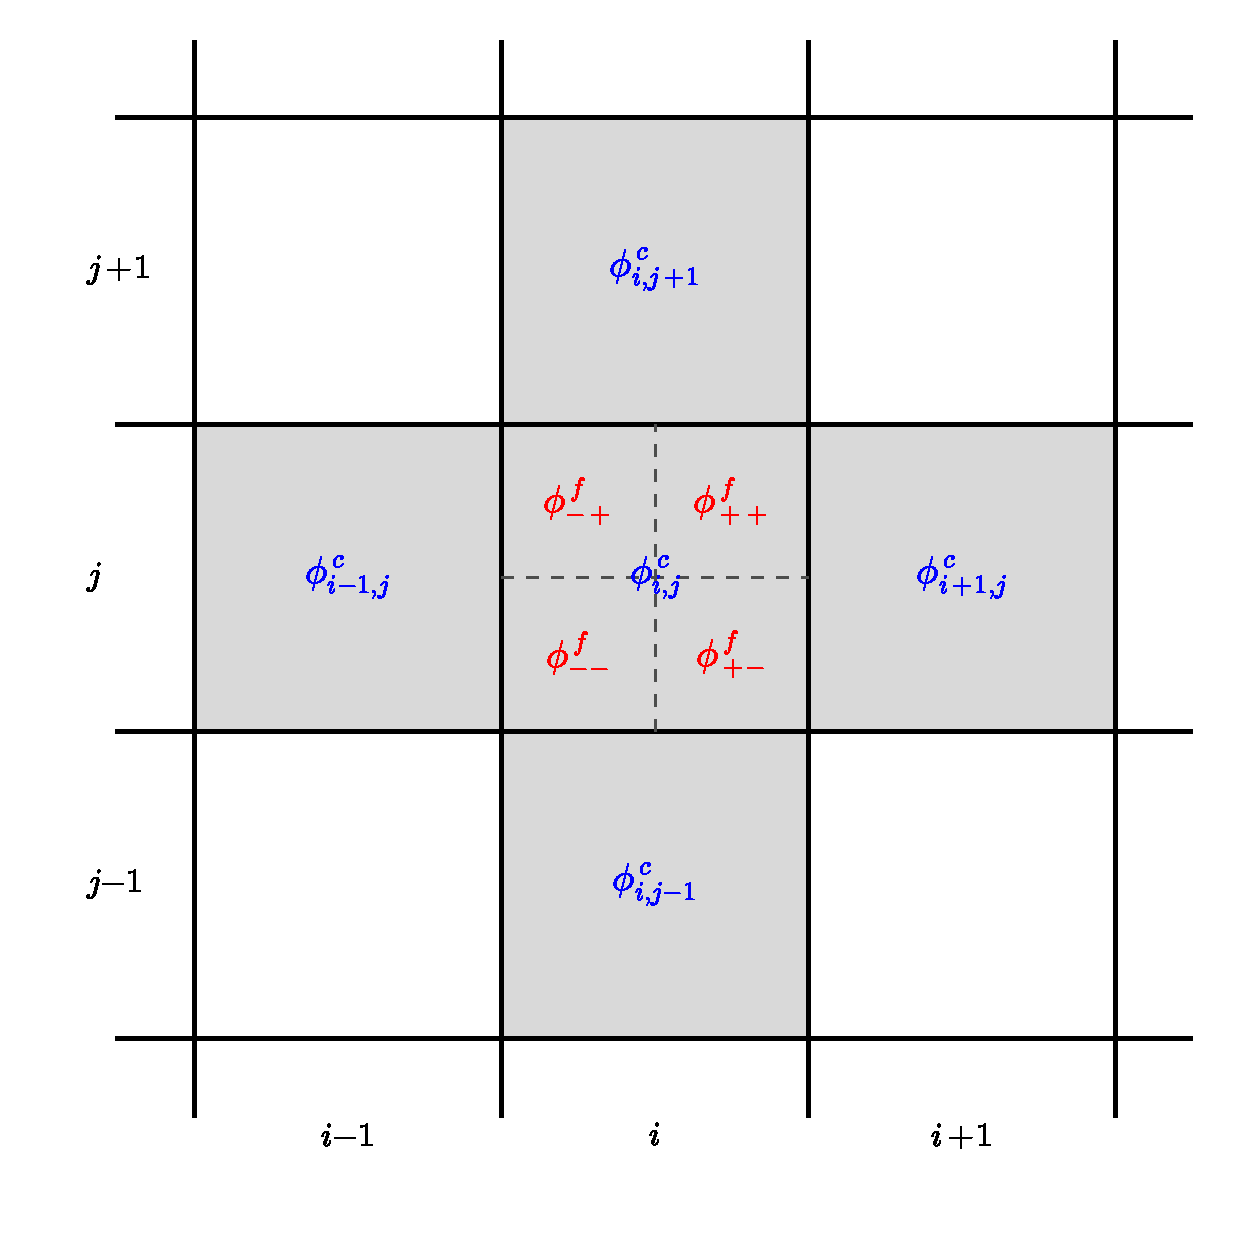
\includegraphics[width=4.0in]{2dgrid-prolong}
\caption[The geometry for 2-d
  prolongation.]{\label{fig:2dgrid-prolong} Four fine cells and the
  underlying coarse grid.  For prolongation, the fine cells in red are
  initialized from a coarse parent.  The gray coarse cells are used in
  the reconstruction of the coarse data.  For restriction, the fine
  cells are averaged to the underlying coarse cell.}
\end{figure}

Restriction from the fine grid to the coarse grid is straightforward.
Since the fine cells are perfectly enclosed by a single coarse cell,
we simply average:
\begin{equation}
\phi_{i,j}^c = \frac{1}{4} ( \phi_{--}^f + \phi_{+-}^f +
                             \phi_{-+}^f + \phi_{++}^f )
\end{equation}

Prolongation requires us to reconstruct the coarse data and use
this reconstruction to determine what the fine cell values are.  For
instance, a linear reconstruction of the coarse data in $x$ and $y$ is:
\begin{equation}
\phi(x,y) = \frac{m_x}{\Delta x} (x - x_i^c) + 
            \frac{m_y}{\Delta y} (y - y_j^c) + \phi_{i,j}^c
\end{equation}
with slopes:
\begin{eqnarray}
m_x &=& \frac{1}{2}({\phi_{i+1,j}^c - \phi_{i-1,j}^c}) \\
m_y &=& \frac{1}{2}({\phi_{i,j+1}^c - \phi_{i,j-1}^c})
\end{eqnarray}
%
When averaged over the coarse cell, $\phi(x,y)$ recovers the average,
$\phi_{i,j}^c$ in that cell (this means that our interpolant is
conservative).  We can evaluate the value in the fine cells by
evaluating $\phi(x,y)$ at the center of the fine cells,
\begin{eqnarray}
x_\pm^f &=& x_i^c \pm \frac{\Delta x^c}{4} \\
y_\pm^f &=& y_j^c \pm \frac{\Delta y^c}{4} \\
\end{eqnarray}
This gives
\begin{equation}
\phi_{\pm\pm}^f = \phi_{i,j}^c \pm \frac{1}{4}m_x \pm \frac{1}{4}m_y
\end{equation}
(Note: you would get the same expression if you averaged $\phi(x,y)$ over
the fine cell.)

There are other options for prolongation and restriction, both of
higher and lower order accuracy.  However, the methods above seem to
work well.

\subsection{Bottom solver}

% this figure can be created with figures/multigrid/mgtower.py
\begin{figure}[t]
\centering
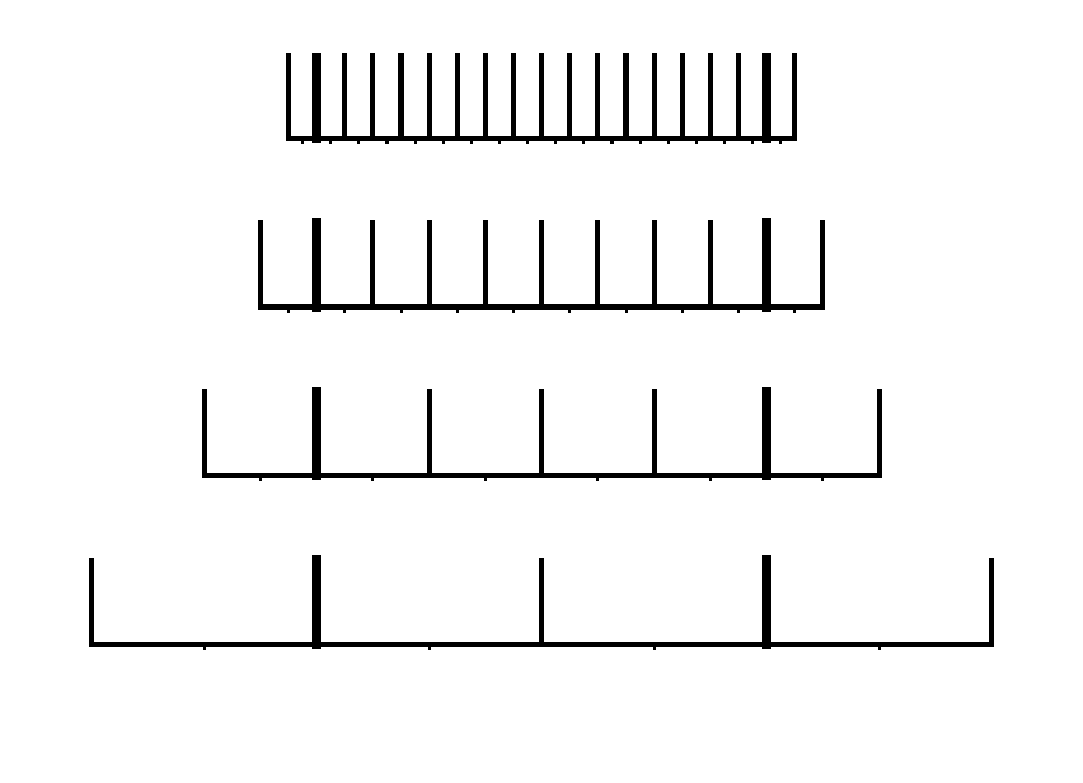
\includegraphics[width=\linewidth]{mgtower}
\caption[A multigrid hierarchy.]{\label{fig:mgtower} Illustration of
  the hierarchy of grids leading to the coarsest 2-zone grid (in
  one-dimension).  Each grid has a single ghost cell to accomodate
  boundary conditions.}
\end{figure}

Once the grid is sufficiently coarse, the linear system is small
enough to be solved directly.  This is the bottom solver operation.
In the most ideal case, where the finest grid is some power of 2, $N_x
= N_y = 2^n$, then the multigrid procedure can continue down until a
$2\times 2$ grid is created (Figure~\ref{fig:mgtower} illustrates this idea
for a one-dimensional grid).  This is the coarsest grid upon which one
can still impose boundary conditions.  With this small grid, just
doing additional smoothing is sufficient enough to `solve' the
problem.  No fancy bottom solver is needed.

For a general rectangular grid or one that is not a power of 2, the
coarsest grid will likely be larger.  For the general case, a linear
system solver like conjugate gradient (or a variant) is used on the
coarsest grid.

\subsection{Boundary conditions throughout the hierarchy}

The general inhomogeneous boundary conditions from
Eqs.~\ref{eq:bc_inhomo_dir} and \ref{eq:bc_inhomo_neum} apply to the
finest level.  But because we are solving the residual equation of the
coarsest levels in the multigrid hierarchy, the boundary conditions on
$Le = r$ are all homogeneous (but of the same type, Dirichlet,
Neumann, or periodic, as the fine level).

Implementing these boundary conditions in your multigrid solver means
that you will have separate actions for the fine level (where
inhomogeneous boundaries may apply) and the coarser levels (where you
will always be homogeneous).



\subsection{Stopping criteria}

Repeated V-cycles are done until:
\begin{equation}
\| r \| < \epsilon \|f\|
\end{equation}
on the finest grid, for some user-input tolerance, $\epsilon$.  Here,
$\|f\|$ is called the {\em source norm}.  If $\|f\| = 0$, then we stop
when
\begin{equation}
\| r \| < \epsilon 
\end{equation}
Picking the tolerance $\epsilon$ is sometimes problem-dependent, and
generally speaking, a problem with a large number of zones will require
a looser tolerance.

The general rule-of-thumb is that each V-cycle should reduce your
residual by about 1 order of magnitude.  It is important that your
bottom solver solves the coarse problem to a tolerance of $10^{-3}$ or
$10^{-4}$ in order for the solver to converge.  Figure~\ref{fig:mgerror}
shows the true and residual errors for $\phi_{xx} = \sin(x)$ as a function
of V-cycle number, illustrating the expected performance.


\begin{figure}
\centering
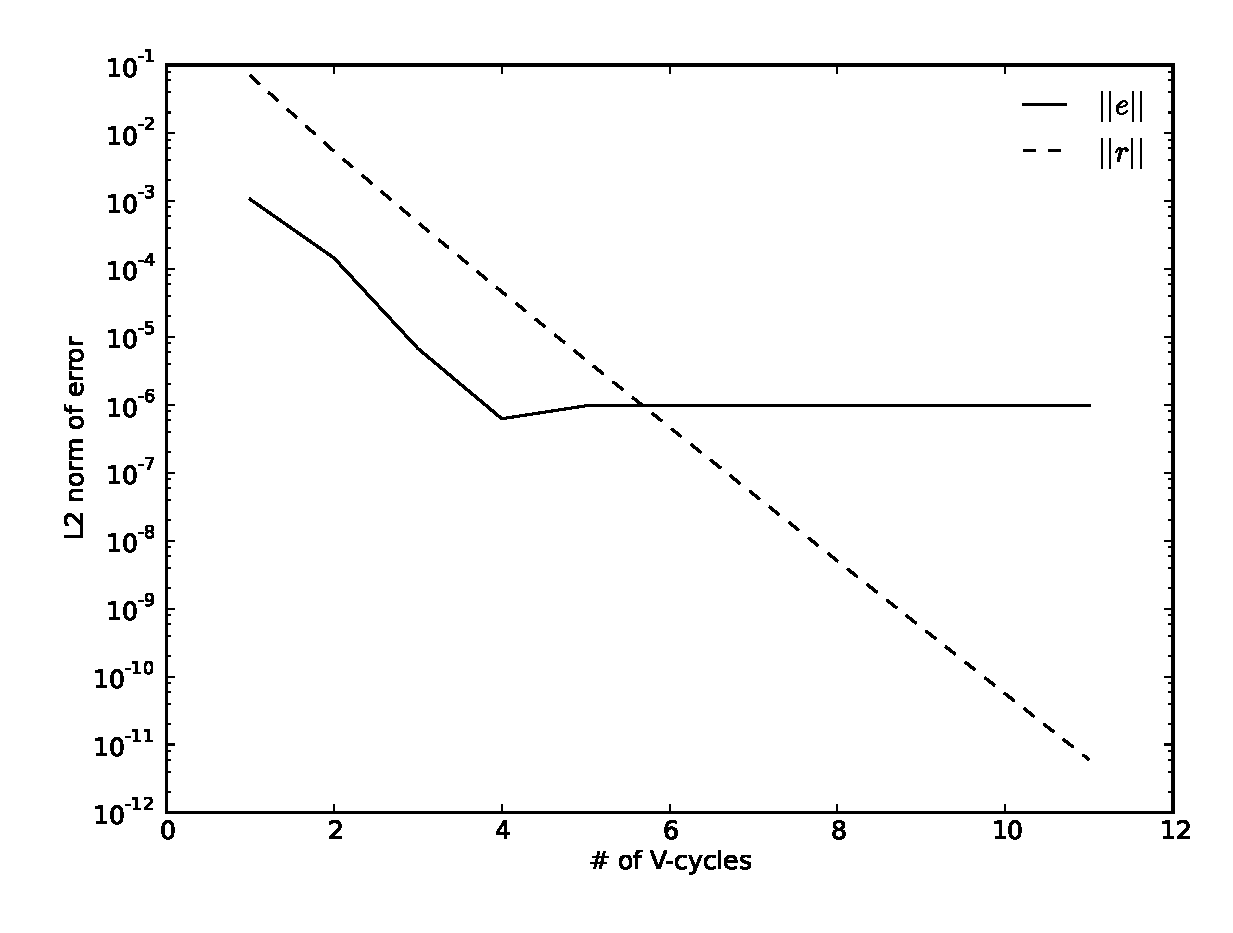
\includegraphics[width=0.85\linewidth]{mg_error_vs_cycle}
\caption[Error in solution as a function of multigrid V-cycle
  number.]{\label{fig:mgerror} Error in the multigrid solution to our
  model problem ($\phi_{xx} = \sin(x)$) as a function of V-cycle.  We
  see that the true error, $\|e\|$ stalls at truncation error while
  the residual error, $\|r\|$ reaches roundoff error, the same
  behavior as seen with smoothing alone (as expected). \\
  \hydroexdoit{\href{https://github.com/zingale/hydro_examples/blob/master/multigrid/mg_test.py}{mg\_test.py}}}
\end{figure}

The overall convergence of the multigrid algorithm is limited by the
discretization of the Laplacian operator used and the implementation
of the boundary conditions.  Figure~\ref{fig:mg:convergence} shows
the error in the solution as the number of zones is increased---demonstrating
second-order convergence for our implementation.

\begin{figure}[t]
\centering
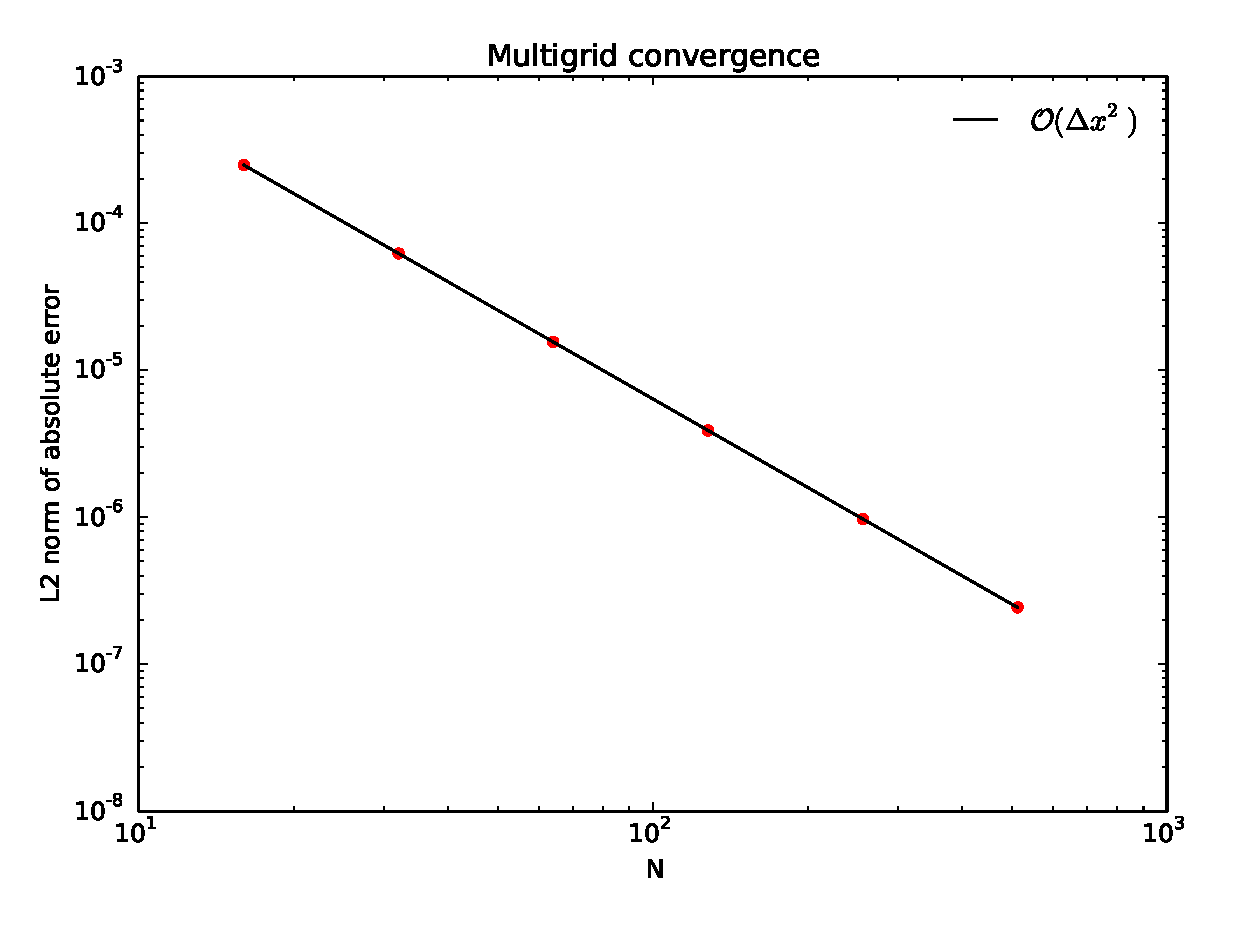
\includegraphics[width=0.85\linewidth]{mg-converge}
\caption[Convergence of the multigrid
  algorithm]{\label{fig:mg:convergence} Convergence of the multigrid
  algorithm. \\ 
  \hydroexdoit{\href{https://github.com/zingale/hydro_examples/blob/master/multigrid/mg_converge.py}{mg\_converge.py}}}
\end{figure}


\section{Going Further}

\label{sec:multigrid:other}

\subsection{Red-black Ordering}

When using domain decomposition to spread the problem across parallel
processors, the smoothing is often done as {\em red-black
  Gauss-Seidel}.  In this ordering, you imagine the grid to be a
checkerboard (see Figure~\ref{fig:rb}).  In the first Gauss-Seidel
pass you update the red squares and in the second, the black squares.
The advantage is that when updating the red, you can be sure that none
of the zones you depend on (the neighboring black zones) will change.
This makes the decomposition parallel.  Note: this works for the
standard 5-point Laplacian.  If you are doing some other operator with
a different stencil, then this decomposition may no longer hold.

% this figure can be created by figures/multigrid/red_black.py
\begin{figure}[t]
  \centering
  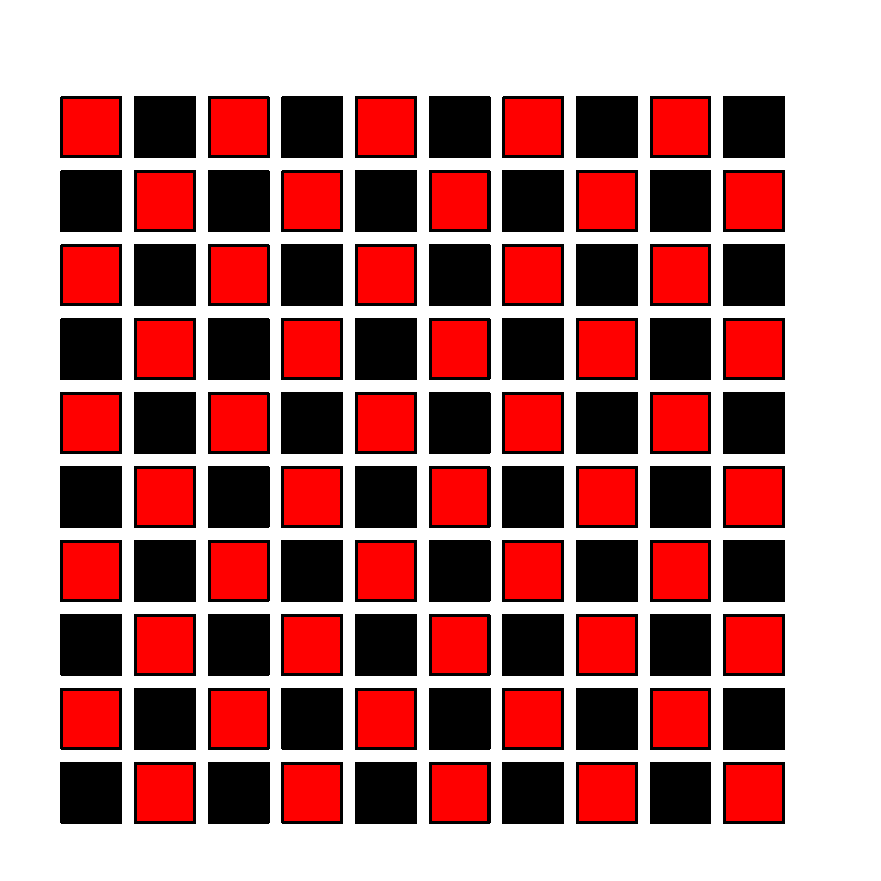
\includegraphics[width=0.6\linewidth]{rb}
  \caption{\label{fig:rb} The red-black ordering of zones}
\end{figure}


\subsection{Solvability}

For $\nabla^2 \phi = f$ with periodic or
Neumann boundaries all around, the sum of $f$ must equal $0$
otherwise the solution will not converge.  Instead, we will simply
find the solution increase each V-cycle.  This is seen as follows:
\begin{equation}
  \int_\Omega f d\Omega = \int_\Omega \nabla^2 \phi d\Omega =
  \int_{\partial \Omega} \nabla \phi \cdot n dS = 0
\end{equation}

For all homogeneous Neumann boundaries, we have $\nabla \phi \cdot dS
= 0$ by construction, so that integral is zero, requiring that the
source integrate to zero.  If the Neumann boundaries are inhomogeneous,
there is still a solvability condition on $f$ based on the sum on
the boundary values.

For all periodic boundaries, we have $\nabla \phi
|_\mathrm{left} = -\nabla \phi |_\mathrm{right}$ on the left and right
boundaries by definition of the periodicity (and similarly for the top
and bottom).  Again this implies that $f$ must integrate to zero.

Sometimes, with periodic boundary conditions all around, you need to
enforce that $f$ integrate to zero numerically to test convergence.
This is discussed in \S~\ref{sec:lm:periodicbcs}.

\subsection{Boundary charges}

For inhomogeneous boundary conditions, {\em boundary charges} can be
used to convert the BCs to homogeneous BCs.  This has the advantage of
allowing the ghost cell filling routines only deal with the
homogeneous case.

Consider the one-dimensional Poisson equation, near the left boundary
our discretized equation appears as:
\begin{equation}
\frac{\phi_\mathrm{lo-1} - 2\phi_\mathrm{lo} + \phi_\mathrm{lo+1}}{\Delta x^2}
 = f_\mathrm{lo}
\end{equation}
Inhomogeneous BCs at the left boundary would give the condition:
\begin{equation}
\phi_\mathrm{lo-1} = 2 \phi_l - \phi_\mathrm{lo}
\end{equation}
Substituting this into the discrete equation, we have:
\begin{equation}
\frac{2 \phi_l - \phi_\mathrm{lo} - 2\phi_\mathrm{lo} + \phi_\mathrm{lo+1}}{\Delta x^2}
 = f_\mathrm{lo}
\end{equation}
Bringing the boundary condition value over to the RHS, we see
\begin{equation}
\frac{- 3\phi_\mathrm{lo} + \phi_\mathrm{lo+1}}{\Delta x^2}
 = f_\mathrm{lo} - \frac{2\phi_l}{\Delta x^2}
\end{equation}
Now the left side looks precisely like the differenced Poisson equation
with homogeneous Dirichlet BCs.  The RHS has an additional `charge' that
captures the boundary value.  By modifying the source term, $f$, in the
multigrid solver to include this charge, we can use the homogeneous 
ghost cell filling routines throughout the multigrid algorithm.
This technique is discussed a bit in~\cite{colellanotes}.

Note that the form of the boundary charge will depend on the form of the
elliptic equation---the expressions derived above apply only for
$\nabla^2 \phi = f$.


\subsection{Norms}

There are several different norms that are typically used in defining
errors on the grid.  The $L_\infty$ norm (or `inf'-norm) is just the
maximum error on the grid:
\begin{equation}
\|e\|_\infty = \max \{ |e_{i,j}| \}
\end{equation}
This will pick up on local errors.  

The $L_1$ norm and $L_2$ norms are more global. 
\begin{eqnarray}
\|e\|_1 &=& \frac{1}{N} \sum_{i,j} |e_{i,j} | \\
\|e\|_2 &=& \left ( \frac{1}{N} \sum_{i,j} |e_{i,j} |^2 \right )^{1/2}
\end{eqnarray}
Generally, the measure in $L_2$ falls between $L_\infty$ and $L_1$.
Regardless of the norm used, if the problem converges, it should
converge in all norms.

For reference, the BoxLib library uses $L_\infty$ in its multigrid solvers.



\subsection{More General Elliptic Equations}

The most general {\em second-order} elliptic equation takes the form:
\begin{equation}
  \alpha \phi + \nabla \cdot (\beta \nabla \phi) +
  \gamma \cdot \nabla \phi + \nabla \cdot (\zeta \phi) = f
\end{equation}
Here, $\gamma$ and $\zeta$ are vectors.  Solving a general elliptic
equation of this form can be accomplished with multigrid using the
same basic ideas here.  The main change is that the smoothing
algorithm and the construction of the residual will need to discretize
the more general operator, and these coefficients will need to
be restricted to the coarser grids (some on edges).  This is explored in
\S~\ref{sec:lm:vcelliptic} for a variable-coefficient Poisson equation:
 \begin{equation}
 \nabla \cdot (\beta \nabla \phi) = f
 \end{equation}
and in \S~\ref{sec:rad:generalelliptic} for an equation with $\zeta = 0$.



